\documentclass{article}

\title{Frekvensresponsen fra scratch}
\author{davipe }
\date{March 2025}

\usepackage{graphicx} % Required for inserting images
\usepackage{amsmath}
\usepackage{amssymb}
\usepackage{amsthm}
\usepackage{url}
\usepackage[a4paper, total={6in, 8in}]{geometry}


\providecommand{\varitem}{} % to keep LaTeX quiet
\makeatletter
\newenvironment{axioms}[1]
 {\renewcommand\varitem[1]{\item[\textbf{#1\arabic{enumi}\rlap{$##1$}.}]%
    \edef\@currentlabel{#1\arabic{enumi}{$##1$}}}%
  \enumerate[label=\textbf{#1\arabic*.}, ref=#1\arabic*]}
 {\endenumerate}
\makeatother

\newcommand{\norm}[1]{\left\lVert#1\right\rVert}


\newtheorem{theorem}{Teorem}
\newtheorem{definition}{Definisjon}
\newtheorem{example}{Eksempel}

\begin{document}

\maketitle

\section{Kompleks analyse og frekvensrespons}

Kompleks analyse dreier seg om funksjoner $f:\mathbb{C} \longrightarrow \mathbb{C}$. Vi trenger noen definisjoner og teoremer fra kompleksanalysen for å utlede frekvensresponsen, hovedsakelig et verktøy for beregning av komplekse integraler som kalles \textit{residyregning}. Til å begynne med må vi derfor legge ned noen grunnleggende definisjoner. Merk at stringens i dette dokumentet vil være generelt svært manglende, og detaljer dessverre må utelates. Likevel prøver vi på en nogenlunde stringent oppbygning.

\subsection{Fundamentale definisjoner}

Vi starter med derivasjon av komplekse funksjoner:

\begin{definition}[Kompleks derivert]
    La $x \in \mathbb{C}$, og $f:\mathbb{C} \longrightarrow \mathbb{C}$ være en kompleks funksjon. Da er den deriverte i punktet $x$ definert som \[f'(x) =  \lim_{z \to x} \frac{f(x) - f(z)}{x - z}. \] Dersom grenseverdien eksisterer, kaller vi f deriverbar.
\end{definition}

\begin{definition}[Holomorf funksjon]
    En funksjon $f:\mathbb{C} \longrightarrow \mathbb{C}$ kalles holomorf hvis den er kompleks deriverbar i et omegn\footnote{\url{https://en.wikipedia.org/wiki/Neighbourhood_(mathematics)}} rundt $x$ for alle $x\in\mathbb{C}$.
\end{definition}

Vi kan også definere noe som minner om en Taylorrekke for komplekse funksjoner, men det har et annet navn og oppfører seg litt annerledes.

\begin{definition}[Laurentrekke]
    La $f: \mathbb{C} \longrightarrow \mathbb{C}$ være en kompleks funksjon, og la $c \in \mathbb{C}$. Laurentrekken til $f$ i $c$ er definert ved \[
    \sum_{n=-\infty}^\infty a_n (z - c)^n,
    \] der $a_n \in \mathbb{C}$.
\end{definition}

Hvordan vi finner koeffisientene er vi nødt til å komme tilbake til litt senere. Merk også at $f(z) = \sum_{n=-\infty}^\infty a_n (z - c)^n$ ikke gjelder for alle funksjoner overalt. Dersom $f(z)$ er lik en Laurentrekke på et omegn rundt ethvert punkt $z \in \mathbb{C}$ kalles den analytisk. Det viser seg faktisk at så lenge en kompleks funksjon er holomorf (altså deriverbar), er den både uendelig deriverbar og analytisk!

Vi har nå diskutert derivasjon av komplekse funksjoner. Men hva med integrasjon? Den første forskjellen mellom $\mathbb{C}$ og $\mathbb{R}$ er at integrasjon ikke lenger gjøres fra $a$ til $b$, men over en \textit{kurve} siden de komplekse tallene kan representeres med et plan.

Det kan være nyttig å starte med definisjonen av linjeintegrasjon av skalarflet i $\mathbb{R}^2$ for å bygge en viss intuisjon.

\begin{definition}[Linjeintegral, $\mathbb{R}^2$]
    Gitt en åpen\footnote{\url{https://en.wikipedia.org/wiki/Open_set}} delmengde $U \subseteq \mathbb{R}^2$, en kurve $L \subset U$ av endelig lengde, en funksjon $f:U \longrightarrow \mathbb{R}$, ofte kalt et skalarfelt, og en kontinuerlig deriverbar parametrisering $\gamma : [0, 1] \longrightarrow L$ er linjeintegralet gitt ved \[
        \oint_\gamma f(z)dz = \int_0^1 f(\gamma(t)) \norm{\gamma'(t)}_2 dt
    \]
\end{definition}

Dette kan tenkes på som at man tar "høyden" i skalarfeltet, langs kurven man integrer over, og integrerer alle høydene. En fin animasjon finnes på wikipedia: \url{https://en.wikipedia.org/wiki/Line_integral#Line_integral_of_a_scalar_field}.

\begin{definition}[Komplekst linjeintegral]
    Gitt en åpen delmengde $U \subseteq \mathbb{C}$, en kurve $L \subset U$ av endelig lengde, en funksjon $f:U \longrightarrow \mathbb{C}$ og en kontinuerlig deriverbar parametrisering $\gamma : [0, 1] \longrightarrow L$ er linjeintegralet gitt ved \[
        \oint_\gamma f(z)dz = \int_0^1 f(\gamma(t)) \gamma'(t) dt
    \]
\end{definition}

Merk at linjeintegralet ikke egentlig krever at parametriseringen skal være kontinuerlig deriverbar, men vi trenger det for å kunne skrive den på den pene formen på høyresiden.

Her kan man ikke anvende den samme intuisjonen som i $\mathbb{R}^2$, men ideen med å integrere over en kurve er den samme, bare at i stedet for reelle tall er verdiene i "skalarfeltet" nå komplekse tall.

Det komplekse linjeintegralet har noen interessante egenskaper:
\begin{example}
    Gitt funksjonen $f:\mathbb{C} \longrightarrow \mathbb{C}$ definert ved $f(z) = (z-c)^n$ for $c \in \mathbb{C}$ og $n \in \mathbb{N}$, kan vi finne linjeintegralet over  enhetssirkelen sentrert i $c$:
    \[\oint_\gamma(z-c)^n dz,\]
    hvor $\gamma:[0, 1] \longrightarrow \mathbb{C}$, $\gamma(t) = e^{2\pi it} + c$. Da er
    \begin{align}
        & \oint_\gamma(z-c)^n dz \\
        =\ & \int_0^1(\gamma(t) - c)^n\gamma'(t) dt \\
        =\ & \int_0^1(e^{2\pi it} + c - c)^n2\pi i e^{2\pi it} dt \\
        =\ & 2\pi i \int_0^1 e^{2\pi it(n + 1)}dt, \\
    \end{align}
    og så lenge $n \neq -1$ kan vi skrive 
    \begin{align}
        & 2\pi i \int_0^1 e^{2\pi it(n + 1)}dt \\
        =\ & 2\pi i \frac{1}{2\pi i(n+1)}e^{2\pi it(n + 1)} \bigg\rvert_{t=0}^1 \\
        =\ & \frac{1}{n + 1} (e^{2\pi i(n + 1)} - 1)
        =\ 0.
    \end{align}
    Hva hvis $n = -1$? Da får vi
        \begin{align}
        & 2\pi i \int_0^1 dt \\
        =\ & 2\pi i. \\
    \end{align}
    Vi kan dermed skrive at, hvis vi integrerer over enhetssirkelen er 
    \[
        \oint_\gamma(z-c)^n dz = \begin{cases}
            0 & n \neq -1 \\
            2 \pi i & n = -1
        \end{cases}.
    \]
\end{example}

Dette eksemplet illustrerer noe som egentlig er mer generelt, men litt for vanskelig å vise. Resultatet gjelder nemlig uavhengig av om vi integrerer over enhetssirkelen eller ikke, så lenge kurven er kontinuerlig deriverbar. 
Dersom vi har en analytisk funksjon (merk at $f(z) = \frac{1}{z}$ ikke er analytisk!) og en lukket kurve blir integralet enda enklere.

\begin{theorem}[Cauchys integralteorem]
    Dersom $\Omega$ er et enkeltsammenhengende\footnote{\url{https://en.wikipedia.org/wiki/Simply_connected_space}} domene og $f:\Omega \longrightarrow \mathbb{C}$ en funksjon som er analytisk (eller holomorf, om du vil) på dette domenet, og $\gamma$ er en lukket sti (altså $\gamma(0) = \gamma(1)$), så er 
    \[
        \oint_\gamma f(z) dz = 0.
    \]
    Med andre ord vil integralet bli null så lenge vi integrerer over en sti som starter og slutter i samme punkt.
\end{theorem}

Når det gjelder beviset av dette refererer jeg heller til wikipedia (\url{https://en.wikipedia.org/wiki/Cauchy%27s_integral_theorem#Proof}) enn å gjøre det selv, fordi det krever resultater fra vektorkalkulus.

En siste kommentar som er av interesse er at det for analytiske funksjoner faktisk viser seg at valget av sti man integrerer over er helt vilkårlig (så lenge man er i domenet til funksjonen, og det er enkeltsammenhengende).

\subsection{Singulariteter og residyer}

Nå som vi kan derivere og integrere, kan vi begynne å jobbe oss fram mot integreringsmetoden som kalles residyregning. Fra Cauchys integralteorem og eksemplet vi regnet ut ser vi at kompleks integrasjon ofte bare blir null, med mindre vi har noe som ikke er analytisk. Derfor er det interessant å snakke om singulariteter.

\begin{definition}[Isolert singularitet]
    Singularitet er vanskelig å definere presist, men vi nøyer oss med å si at de er punkter hvor en funksjon $f:\mathbb{C} \longrightarrow \mathbb{C}$ slutter å være definert. En singularitet kalles isolert hvis det finnes en åpen disk\footnote{\url{https://en.wikipedia.org/wiki/Disk_(mathematics)}} $D_r(c)$ med sentrum i $c$, slik at $f$ er holomorf i området $D_r(c) \setminus \{c\}$, altså disken med singularitetspunktet fjernet.
\end{definition}

\begin{definition}[Simpel pol]
    En simpel pol er en pol ($z \in \mathbb{C}$ slik at $\frac{1}{f(z)} = 0$) av orden $1$ (tenk på orden som eksponenten i telleren til $f(z)$).
\end{definition}

En isolert singularitet kan altså tenkes på som en singularitet som ikke har andre singulariteter like ved. Et eksempel finnes i funksjonen $f(z) = \frac{1}{z}$, denne har en isolert singularitet i $z = 0$, da funksjonen er udefinert i dette punktet (singulariteten er faktisk også en simpel pol!). Vi kan nå definere en type funksjon som er "nesten holomorf".

\begin{definition}[Meromorf funksjon]
    En funksjon $f:\mathbb{C} \longrightarrow \mathbb{C}$ kalles meromorf hvis den er holomorf på hele $\mathbb{C}$, bortsett fra et sett med isolerte singulariteter. 
\end{definition}

\begin{definition}[Residy]
    Gitt en meromorf funksjon $f:\mathbb{C} \longrightarrow \mathbb{C}$ og en isolert singularitet $c \in \mathbb{C}$ er residyet til $c$ gitt ved den unike verdien $R$ slik at $f(z) - \frac{R}{z - c}$ har en holomorf antiderivert i en punktert disk $0 < |z - c| < \delta$. Residyet betegnes ofte $\mathrm{res}(f, c)$.
\end{definition}

Grunnen til at residyer navngis slik som de gjør (Residy minner veldig om "rest") er at residyene representerer det som er "til overs" når vi har integrert over alle de analytiske delene av domenet. Som vi vet fra Cauchy's integralteorem blir dette gjerne null, og da er residyene det som er til overs.
Måten det er definert på kan gjøre at residyer virker vanskelig å forstå og bruke, men heldigvis har residyer en fin egenskap som gjør at de er mye enklere å beregne enn man kanskje skulle tro, som vi nå skal utlede.

\begin{theorem}
    Residyet til en meromorf funksjon $f:\mathbb{C} \longrightarrow \mathbb{C}$ i et punkt $c$ er gitt ved $a_{-1}$, hvor $a_{-1}$ er "minus første" ledd i Laurentrekken til $f$ rundt $c$. 
\end{theorem}

\begin{proof}
    Vi har residyet $R$ slik at funksjonen $f(z) - \frac{R}{z - c}$ har holomorf antiderivert på disken rundt $c$. Derfor setter vi (på disken) den antideriverte 
    \[
        F(z) = \sum_{n = -\infty}^{\infty} a_n (z - c)^n.
    \]
    Vi kan nå se at
    \begin{align}
        F'(z) = & \sum_{n = -\infty}^{\infty} n a_n (z - c)^{n - 1} = f(z) - \frac{R}{z - c} \\
        = & \sum_{n = -\infty}^{\infty} n a_n (z - c)^{n - 1} + \frac{R}{z - c} = f(z).
    \end{align}
    Vi velger nå en sti $\gamma$ som ligger inni disken, slik at vi kan bytte ut $f(z)$ med Laurentrekken. Da blir integralet av høyresiden 
    \begin{align}
        \oint_\gamma f(z) dz = \oint_{\gamma} \sum_{n = -\infty}^{\infty} a_n (z - c)^{n} dz,  
    \end{align}
    hvor vi drister oss til å bytte på summen, og ser nøye på integralene og ser at
    \begin{align}
        & \sum_{n = -\infty}^{\infty} a_n \oint_{\gamma} (z - c)^{n} dz \\
        =\ & \sum_{n = -\infty}^{\infty} a_n \begin{cases}
            0 & n \neq -1 \\
            2 \pi i & n = -1 \\
        \end{cases} \\
        =\ & 2\pi i.
    \end{align}
    Hva skjer på venstresiden? Merk at i Laurentrekken er leddet tilhørende $n = 0$ forsvunnet fordi vi ganger med $n$ foran. Ved et lignende argument som over får vi derfor at 
    \begin{align}
        & \oint_{\gamma} \sum_{n = -\infty}^{\infty} n a_n (z - c)^{n - 1} + \frac{R}{z - c} dz \\
        =\ & \sum_{n = -\infty}^{\infty} n a_n \oint_{\gamma}  (z - c)^{n - 1} dz + \oint_{\gamma} \frac{R}{z - c} dz \\
        =\ & 2 \pi iR.
    \end{align}
    Dermed, når vi setter alt dette sammen får vi at
    \[
        R = a_{-1}
    \]
\end{proof}

For å beregne residyer må vi altså lage en Laurentrekke og se hva koeffisisenten tilsvarende $n = -1$ er. Et enkelt eksempel:

\begin{example}
    Gitt funksjonen $f:\mathbb{C} \longrightarrow \mathbb{C}$, hvor $f(z) = z^k$, $k\in\mathbb{Z}$, er residyet i $c = 0$ gitt ved \[
        \mathrm{res}(f, 0) = \begin{cases}
            0 & k \neq -1 \\
            1 & k = -1
        \end{cases}.
    \]
\end{example}

Det finnes også en enda enklere måte å beregne residyet på dersom singulariteten $c$ er en simpel pol.

\begin{theorem}
    Residyet til en meromorf funksjon $f:\mathbb{C} \longrightarrow \mathbb{C}$ i en simpel pol $c$ er gitt ved 
    \[
        \mathrm{res}(f, c) = \lim_{z \to c} (z - c) f(z)
    \]
\end{theorem}

\begin{proof}
    Siden $f$ er meromorf og singulariteten er isolert, kan vi skrive en lokal Laurentrekke slik at $f(z) = \sum_{n=-\infty}^{\infty}$. Siden polen er simpel vet vi at for $n < -1$ er $a_n = 0$. Dermed kan vi si 
    \[
        f(z) = \sum_{n=0}^{\infty} a_n(z - c)^n + \frac{a_{-1}}{z - c}.
    \]
    Dermed er 
    \begin{align}
        \lim_{z \to c} (z - c)f(z) =& \lim_{z \to c} (z - c) \bigg( \sum_{n=0}^{\infty}a_n(z - c)^n + \frac{a_{-1}}{z - c} \bigg) \\
        = &  \lim_{z \to c} \bigg( \sum_{n=0}^{\infty}a_n(z - c)^{n+1} + a_{-1} \bigg) \\
        = & \bigg( \sum_{n=0}^{\infty}a_n(c - c)^{n+1} + a_{-1} \bigg)
        = a_{-1}
        = \mathrm{res}(f, c)
    \end{align}
\end{proof}

Dette funker bra hvis vi har simple poler, men hva om vi har poler av orden $n$? Det finnes heldigvis et resultat for dette tilfellet også. Beviset viser seg faktisk å være like enkelt som i forrige tilfelle! (merk at notasjonens slapphet til en viss grad er økt i dette tilfellet)

\begin{theorem}
    Residyet til en meromorf funksjon $f:\mathbb{C} \longrightarrow \mathbb{C}$ i en pol $c$ av orden $m$ er gitt ved 
    \[
        \mathrm{res}(f, c) = \lim_{z \to c} \frac{1}{(m - 1)!} \frac{d^{m - 1}}{dz^{m - 1}} (z - c)^m f(z).
    \]
\end{theorem}

\begin{proof}
    Vi kan nå anta at $f$ kan skrives som en Laurentrekke i et omegn av $c$. Nå blir eneste forskjellen at for $n < -m$ blir $a_n=0$. Dermed er 
    \[
        f(z) = a_{-m}(z - c)^{-m} + \cdots + a_{-1} (z-c)^{-1} + \cdots,
    \]
    så ganging på begge sider gir
    \[
        f(z)(z - c)^{m} = a_{-m} + \cdots + a_{-1} (z-c)^{m - 1} + a_0 (z - c)^m + \cdots.
    \]
    Deretter deriverer vi $m - 1$ ganger
    \[
        \frac{d^{m - 1}}{dz^{m - 1}} f(z)(z - c)^{m} = (m - 1)!a_{-1} + a_0 (z - c) + \cdots,
    \]
    og i grenseverdien forsvinner enda flere ledd slik at

    \[
        \lim_{z \to c} \frac{1}{(m - 1)!} \frac{d^{m - 1}}{dz^{m - 1}} (z - c)^m f(z) = a_{-1} = \mathrm{res}(f, c).
    \]
\end{proof}

Residyer kan brukes når vi integrerer i det komplekse planet, noe vi snart skal få bruk for. Merk at i definisjonen under er detaljene svært forenklet i et forsøk på å gjøre leseren mindre avskrekket.

\begin{theorem}[Residyteoremet]
    Gitt en liste punkter $Z_1, ... , Z_n$ (disse er ofte singulariteter), en holomorf funksjon $f:\mathbb{C} \longrightarrow \mathbb{C}$ og en lukket kurve $\gamma$ er linjeintegralet gitt ved \[
    \oint_\gamma f(z) dz = 2 \pi i \sum_{i = 1}^n I(\gamma, Z_i) \mathrm{res}(f, Z_i),
    \] hvor $I(\gamma, Z_i)$ representerer vindingstallet\footnote{\url{https://en.wikipedia.org/wiki/Winding_number}} til $\gamma$ rundt $Z_i$.
\end{theorem}

\begin{figure}
        \centering
        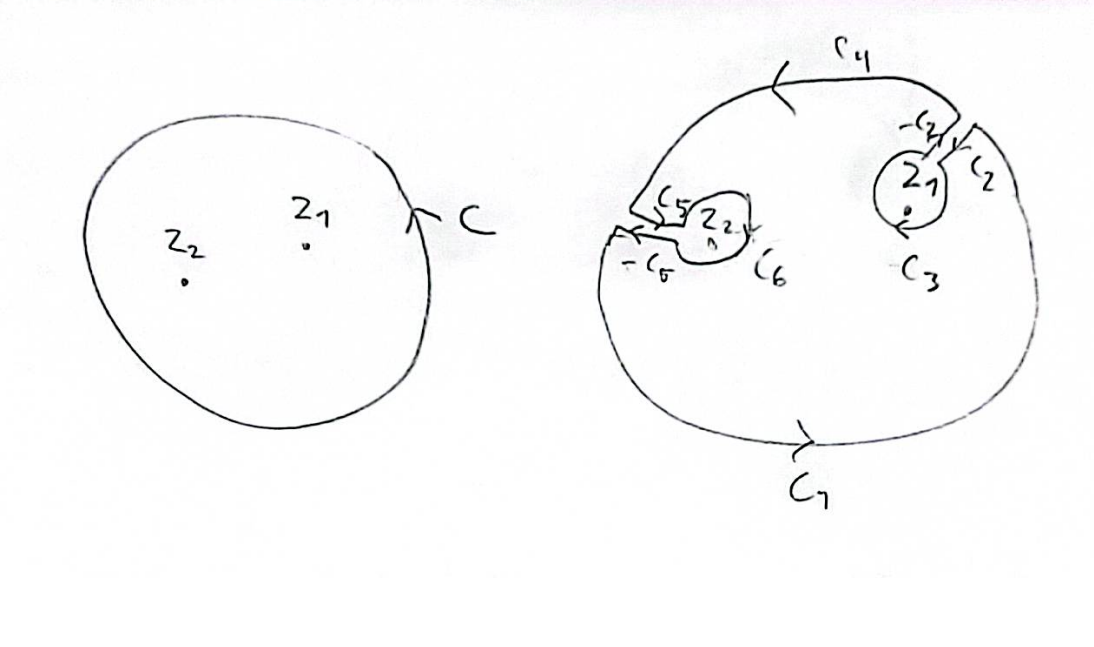
\includegraphics[width=\linewidth]{images/residuethm.png}
        \caption{Finurlig valgte stier for residyteoremet.}
        \label{fig:residuethm}
\end{figure} 

\begin{proof}
    I figur \ref{fig:residuethm} har vi tegnet inn en kurve med to singulariteter ($Z_1$ og $Z_2$) (beviset fungerer også for $n$ singulariteter), hvor vi på høyresiden har kuttet opp kurven slik at singularitetene havnet utenfor kurven. Vi har nå at 
    \[
        \Tilde{C} = C_1 + C_2 - C_3 - C_2 + C_4 + C_5 - C_6 - C_5
    \]
    på høyresiden, og på venstresiden $C = C_1 + C_4$. Siden $f$ er analytisk unntatt der det er poler er integralet (ved Cauchy's integralteorem)
    \[
        \oint_{\Tilde{C}} f(z) dz = \oint_{C_1 + C_2 - C_3 -C_2 + C_4 + C_5 - C_6 - C_5} f(z) dz = 0.
    \]
    Vi dropper $C_2$ og $C_5$ da disse blir lagt til og trukket fra, og set at
    \[
    \oint_{C_1 + C_4} f(z) dz = \oint_{C_3 + C_6} f(z) dz.
    \]
    Vi lager nå Laurentrekker rundt singularitetene $Z_1$ og $Z_2$ slik at 
    \begin{align}
        & \oint_{C_3} f(z) dz \\
        =\ & \sum_{n=-\infty}^{\infty} \oint_{C_3} a_n (z - Z_1)^n dz \\ 
        =\ & 2\pi i a_{-1} \\ 
        =\ & 2\pi i \ \mathrm{res}(f, Z_1).
    \end{align}
    På samme vis blir
    \begin{align}
        & \oint_{C_6} f(z) dz \\
        =\ & 2\pi i \ \mathrm{res}(f, Z_2).
    \end{align}
    Siden $C = C_1 + C_4$ blir da 
    \[
        \oint_C f(z) dz = 2\pi i (\mathrm{res}(f, Z_1) + \mathrm{res}(f, Z_2)).
    \]
    Beviset er enkelt (men kjedelig) å generalisere til $n$ poler.
\end{proof}

Dersom det er uklart hvor vindingstallet har blitt av i beviset over, så er svaret at vindingstallet $I(\gamma, Z_i) = 1$. Dette gjelder generelt så lenge kurven $\gamma$ går rundt punktet $Z_i$ kun én gang, og mot klokken. I resten av teksten kommer vi ikke til å se vindingstallet igjen, fordi vi er i nettopp dette tilfellet.

Med andre ord kan vi beregne linjeintegraler i det komplekse planet ved å summere residyer. Nå som residyregningen er i boks, skal vi snart benytte dette til å beregne inversen av laplaceomvendingen, men først må vi definere noen sentrale begreper fra systemteoriens verden.

\subsection{Utledningen}

\begin{definition}[Signal]
    Et signal er en funksjon $x:\mathbb{R} \longrightarrow \mathbb{R}$ slik at $x(t) = 0 \ \forall \ x < 0$.
\end{definition}

\begin{definition}[Laplaceomvending]
    Gitt et signal $x$ er laplaceomvendingen gitt ved \[
        X(s) := \int_0^\infty x(t) e^{-st}dt,
    \]
    hvor $s\in\mathbb{C}$. 
\end{definition}

Her følger noe som kanskje ikke er fullt så kjent, nemlig inversen til Laplaceomvendingen.

\begin{definition}[Invers Laplaceomvending]
\label{laplaceinverse}
    Gitt en funksjon $X:\mathbb{C} \longrightarrow \mathbb{C}$ er invers-laplaceomvendingen gitt ved \[
        x(t) := \frac{1}{2 \pi i} \lim_{T\to\infty} \int_{a - iT}^{a + iT} X(s) e^{st}ds,
    \]
    hvor $a$ er større enn realdelen til alle singulariteter for $X$.
\end{definition}

Det er selvfølgelig et teorem som sier at laplace og invers-laplace kansellerer, men det krever en del detaljer jeg ikke har lært selv enda. Dersom det likevel er interesse for å lese og prøve å forstå beviset, finner du det på math stackexchange\footnote{\url{https://math.stackexchange.com/questions/2926685/proof-of-inverse-laplace-transform}}.

Med disse verktøyene vi nå har under beltet kan vi endelig vise hvorfor uttrykket for frekvensresponsen er slik som det er.

% NO
\begin{theorem}[Frekvensresponsen]
    Gitt et signal $u(t) = \sin(\omega t)$, en transferfunksjon (signal) $h:\mathbb{R} \longrightarrow \mathbb{R}$ er steady-state responsen et signal $y(t) = (h * u)(t)$, hvor $*$ betegner konvolusjon gitt ved $y(t) = |H(i\omega)|sin(\omega t + \angle H(j\omega))$, hvor $H(s)$ er Laplaceomvendingen til $h(t)$.
\end{theorem}

\begin{figure}
        \centering
        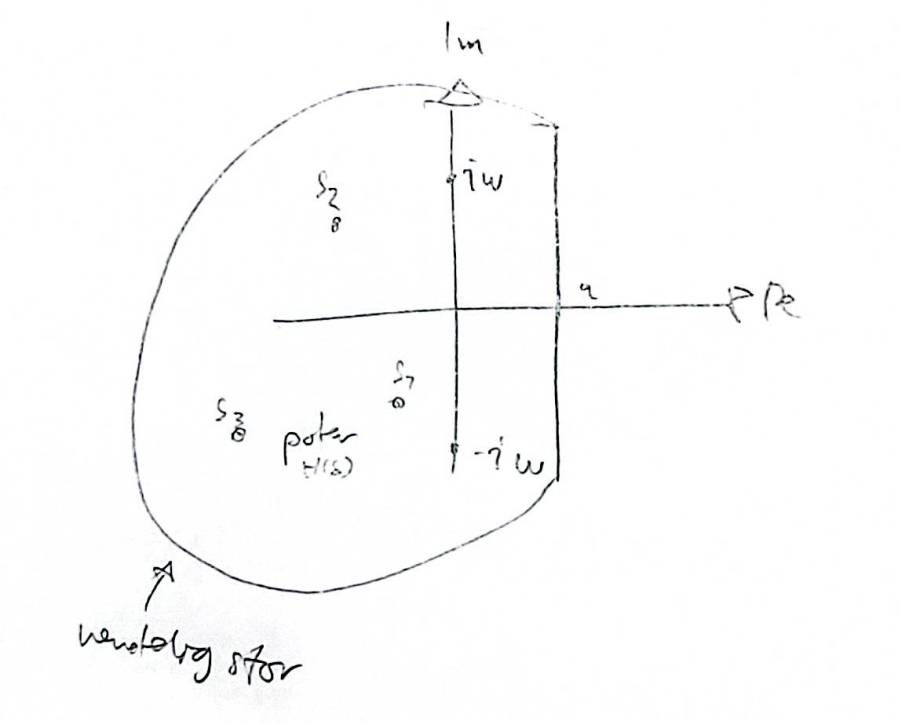
\includegraphics[width=\linewidth]{images/freqresp.png}
        \caption{Integrasjonssti for invers laplaceomvending. Polene til $H(s)$ er i venstre halvplan.}
        \label{fig:freqresp}
\end{figure} 

\begin{proof}
    Merk først (sjekk gjerne selv) at $Y(s) = H(s) X(s)$, altså at Laplaceomvending gjør konvolusjon om til multiplikasjon. I tillegg er \[
        X(s) = \frac{\omega}{s^2 + \omega^2},
    \] så vi får 
    \[
        Y(s) = H(s) \frac{\omega}{s^2 + \omega^2}.
    \]
    Nå anvender vi definisjonen av Laplace-invers, slik at
    \[
     y(t) = \frac{1}{2\pi i} \lim_{T\to\inf} \int_{a-iT}^{a+iT} Y(s) e^{st} ds.
    \]
    For å beregne dette integralet tenker vi at vi har en sti som går gjennom den vertikale linjen i $\mathrm{Re}(z) = a$, og så en uendelig stor halvsirkel i venstre halvplan, som vist i figur \ref{fig:freqresp}. Vi har singulariteter i $i\omega$, $-i\omega$ og muligens flere poler fra $H(s)$. Merk at dersom vi ikke antar at disse ligger i venstre halvplan, vil ikke steady-state responsen eksistere, og derfor må vi anta dette. Ved residyteoremet får vi da at
    \[
    y(t) = \mathrm{res}(Y(s)e^{st}, iw) + \mathrm{res}(Y(s)e^{st}, -iw) + \sum_{i = 1}^n \mathrm{res}(Y(s)e^{st}, s_i).    
    \]
    Vi har simple poler i $i\omega$ og $-i\omega$, og antar at alle andre poler i transferfunksjonen har poler av høyest orden $m$. Da blir residyene 
    \[
    y(t) = \frac{H(i\omega)\omega e^{i\omega t}}{2i\omega} + \frac{H(-i\omega)\omega e^{-i\omega t}}{-2i\omega} + \sum_{i = 1}^n \lim_{s \to s_i} \frac{1}{(m  - 1)!} \frac{d^{m - 1}}{dz^{m  -1}} \frac{(s-s_i)^m H(s)\omega e^{ts}}{s^2 + \omega^2}.
    \]
    Vi ser på steady-state respons, og vi antar naturligvis da at polene til $H(s)$ er i venstre halvplan. Siden vi ser på steady state respons antar vi at $t$ vokser og vet dermed at faktoren $e^{ts}$ kommer til å dominere de andre (eksponentialfunksjonen vokser/synker raskere enn alle polynomer), og følgelig er bidraget polene til transferfunksjonen null i steady-state. Vi står da igjen med
    \begin{align}
        y_s(t) & = H(i\omega)\frac{e^{i\omega t}}{2i} - H(-i\omega)\frac{e^{-i\omega t}}{2i} \\
        & = |H(i\omega)| \frac{e^{i(\omega t + \angle H(iw))} - e^{-i(\omega t + \angle H(iw))}}{2i} \\
        & = |H(i\omega)| sin(\omega t + \angle H(j \omega)).
    \end{align}
\end{proof}

\section{Avslutning}

Hvis du leste helt hit, takk! Jeg begynte å skrive dette dokumentet da jeg ble spurt av en uvitende førsteklassing om hvordan man utleder frekvensresponsen, hvor de også viste meg en ganske utilfredsstillende utledning gitt av en professor på ITK.
Jeg, i mitt hovmod antok at oppgaven var enkel og lovte å levere en full utledning av hvorfor frekvensresponsen er som den er. Dette viste seg å være vanskeligere enn jeg først hadde trodd. Det tok ikke særlig lang tid å finne løsningen i Balchen, Andresen og Foss' regtek-bok, men for å bevare matematisk stringens anså jeg det som nødvendig å inkludere noen fundamentale resultater fra kompleks analyse (et fag jeg selv ikke engang har hatt, jeg har hovedsakelig lent meg på wikipedia og andre nettressurser).
Det hele førte til en lang arbeidsprosess hvor jeg ble tvunget til å lære residyregning, laplaceinversomvending og deler av kompleks analyse på nytt, noe jeg er veldig takknemlig for. Når det er sagt vil jeg be om at ingen noen gang spør meg om å gjøre noe slikt igjen, da dette har tatt \textit{mye} lengre tid enn jeg hadde forventet at det skulle ta (jeg har fullstending begått alt jeg skulle gjøre av skolerbeid).

\end{document}
